\section{World Level: Are Road Claims Identifiable?}
\label{sec:world}

\subsection{Data and protocol}
\label{sec:data}
The Passive Vehicular Sensors (PVS) dataset~\cite{menegazzo2021pvs} has nine trips in which three vehicle--driver pairs each drove the same three routes (10.7, 11.6 and 13.8~km).
Each vehicle carries a left and a right logger. Each logger has IMU modules on the dashboard and above and below the suspension, plus its own GNSS receiver.
Every sample is labelled with speed bumps, surface type and the road quality of each side (good, regular, bad).

We use the left logger's dashboard module, the closest proxy for a phone in a holder (the modules are not phones), and the left-side quality label. The right logger provides the noise floor and a replication.
Each trip's GNSS fixes are matched in time order to the first vehicle's track within a forward window. The other vehicles' fixes lie a median 1.5--3.8~m from that track, and 97.9--99.3\% of samples are matched.
Routes are cut into 100~m stretches.
A place enters the primary analysis if all three vehicles drove it at a mean speed of at least 5~m\,s$^{-1}$, RoadScribe's floor for road values. This holds for 310 of the 361 places; Section~\ref{sec:calibration} also reports all 361.
The quality labels agree across the three trips of a route (weighted $\kappa=0.93$), so they serve as a vehicle-independent reference.

\emph{Pre-specification.}
Each analysis in Table~\ref{tab:prereg} was written down, with its hypotheses and thresholds, and committed to the project repository before it was run. Failed hypotheses are reported as such.
The commits are timestamps in an author-controlled repository, not entries in an independent registry, so we offer them for transparency rather than as a guarantee.
RoadScribe's default $\gamma=0.35$ predates all of them: it was estimated on the same trips during development (across places, on asphalt) and fixed in the configuration on 2026-11-03.
Analyses not listed in Table~\ref{tab:prereg} are labelled exploratory.

\emph{Uncertainty.}
Intervals come from a block bootstrap with 2{,}000 resamples. The resampling units are contiguous 1~km blocks of ten places within each route (12, 10 and 10 blocks).
With only three vehicles, these intervals do not reflect the sampling of vehicles.

\begin{table*}[t]
\caption{Analyses specified in advance: written down and committed to the project repository before they were run (times IST, 2026). P7 was added after a first review round.}
\label{tab:prereg}
\centering
\footnotesize
\setlength{\tabcolsep}{4pt}
\begin{tabular}{@{}lll>{\raggedright\arraybackslash}p{6.8cm}>{\raggedright\arraybackslash}p{5.2cm}@{}}
\toprule
ID & Committed & Commit & Question & Outcome \\
\midrule
P1 & 11-12 00:21 & \texttt{6a135d8} & Are ride and road classes vehicle-invariant? & Main hypothesis (road classes not invariant) held; 2 of 5 others did not \\
P2 & 11-12 00:27 & \texttt{624fee0} & Does a spectral vehicle model (Eq.~\ref{eq:scr}) remove the vehicle share? & 3 of 4 held; speed dependence not reduced \\
P3 & 11-12 00:31 & \texttt{081c9dc} & Does that model predict an unseen vehicle's ride better than scalar gains? & Neither hypothesis held \\
P4 & 11-12 14:56 & \texttt{265e705} & Does calibration on shared roads (Eq.~\ref{eq:cal}) restore agreement? & All 4 held \\
P5 & 11-12 16:16 & \texttt{5934f72} & Does plan--ground--realize training help the model? & 2 of 4 held \\
P6 & 11-13 00:23 & \texttt{0bda5ac} & With the targets fixed, does adding the stated values to the input help? & 3 of 4 held \\
P7 & 11-13 00:43 & \texttt{5891276} & Noise floor, data efficiency, held-out accuracy, speed floor & All 6 held \\
\bottomrule
\end{tabular}
\end{table*}

\subsection{Agreement across vehicles}
\label{sec:invariance}
Ride classes \emph{should} differ between vehicles. Road classes are worded as properties of the road (``the surface is in fair condition''), so they should agree.
They do not (Table~\ref{tab:invariance}).
The road class differs between two vehicles at the same place in 76\% of pairs, and all three vehicles agree at only 4.5\% of places.
Net of place and log speed, the vehicle accounts for 18.2\% of the variance of the log road value.
Shuffling vehicle labels within places 1{,}000 times gives a vehicle share of 0.06\% (99th percentile 0.27\%).
The residual, which contains any place-by-vehicle interaction, is only 2.1\% of the variance, so the vehicles differ mainly by a constant factor.

Two dashboard modules in the \emph{same} vehicle on the \emph{same} pass agree at $\kappa=0.98$. They never differ by more than one class, and the side explains 0.03\% of the variance. Cross-vehicle disagreement is therefore not measurement noise.
The right logger replicates the cross-vehicle result (vehicle share 17.8\%, $\kappa=0.72$).
The size of the vehicle signature depends on the mount (exploratory): 2.9\% above the suspension ($\kappa=0.86$) and 11.8\% below it ($\kappa=0.60$). The dashboard is the worst of the three.

\begin{table*}[t]
\caption{Agreement of per-stretch classes across the three vehicles at 310 places (dashboard IMU). $\kappa$: mean pairwise quadratic-weighted kappa of the six classes. Vehicle share: unique variance explained by the vehicle in $\log$ value $\sim$ place + vehicle + $\log\bar v$. Brackets: 95\% block-bootstrap intervals. Last row: the two modules of the same vehicle on the same pass.}
\label{tab:invariance}
\centering
\footnotesize
\setlength{\tabcolsep}{6pt}
\begin{tabular}{@{}lcccc@{}}
\toprule
Claim & $\kappa$ & all three agree & pairs differ & vehicle share \\
\midrule
Ride class, $a_v$ & 0.66 [0.53, 0.72] & 9.7\% & 66\% & 18.8\% [14.8, 27.4] \\
Road class, $\tilde a_w$ ($\gamma=0.35$) & 0.72 [0.60, 0.76] & 4.5\% [2.6, 6.7] & 76\% & 18.2\% [14.3, 27.5] \\
Road class, calibrated (Eq.~\ref{eq:cal}) & 0.96 [0.93, 0.97] & 64.8\% [58.7, 70.9] & 24\% & $<$0.1\%\textsuperscript{a} \\
\midrule
Same vehicle, left vs.\ right module & 0.98 [0.97, 0.98] & -- & 7.8\% & 0.03\% (side) \\
\bottomrule
\end{tabular}

\smallskip
{\scriptsize\textsuperscript{a}\,Near zero largely by construction: the gains come from the other routes and hardly vary between routes.}
\end{table*}

\subsection{Speed}
\label{sec:speed}
Pooled across places, vibration \emph{falls} with speed (Fig.~\ref{fig:speed}, slope $-0.64$), because the rough places are driven slowly.
Within a place, net of vehicle, it rises (slope $+0.86$; difference 1.50 [1.26, 1.64]).
The reversal comes mostly from surface type. Within each surface the pooled slope is positive (asphalt $+0.16$, cobblestone $+0.54$, dirt $+1.36$; exploratory), though on asphalt it is still far below the within-place $+0.96$.
RoadScribe's $\gamma=0.35$ was estimated in the across-place way. With it, the road value still rises with speed at a fixed place (slope 0.51).
An elasticity for decoupling has to come from repeated passes over the same places, as in Eq.~\eqref{eq:fe}.

\begin{figure*}[t]
\centering
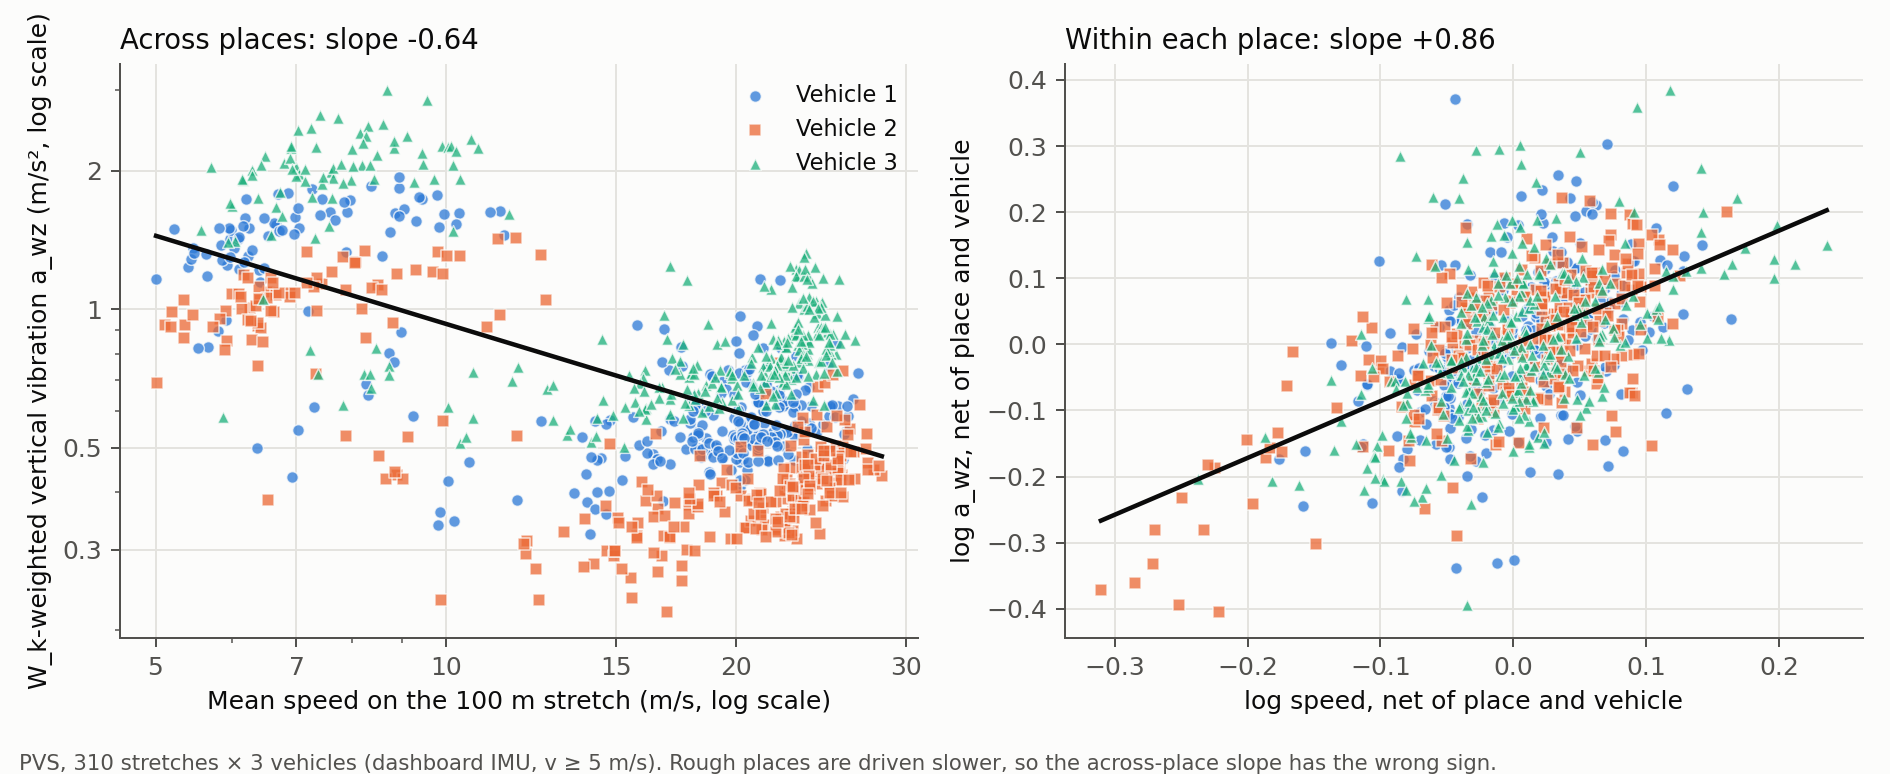
\includegraphics[width=0.78\textwidth]{fig_speed.png}
\caption{Speed elasticity of dashboard vibration at 310 places, three vehicles ($v\ge5$~m\,s$^{-1}$). Left: across places (pooled OLS, slope $-0.64$); rough places are driven slowly. Right: within places, net of place and vehicle (partial-regression plot of Eq.~\eqref{eq:fe}, slope $+0.86$).}
\label{fig:speed}
\end{figure*}

\subsection{Calibration on shared roads}
\label{sec:calibration}
We calibrate leave one route out: $\hat\gamma$ and $\hat g_c$ come from Eq.~\eqref{eq:fe} on the other two routes, and the held-out route gets Eq.~\eqref{eq:cal}.
The estimates hardly change with the held-out route: $\hat\gamma=0.87$--$0.88$, and the gains are about $+0.04$, $-0.36$ and $+0.32$ log units. At the same place and speed, the third vehicle reads almost twice as high as the second.
After calibration, cross-vehicle $\kappa$ rises from 0.72 to 0.96 (difference [0.20, 0.33]; Table~\ref{tab:invariance}), closing 92\% of the gap to the same-vehicle floor, and on the right logger it rises from 0.72 to 0.95.
The road value also stops rising with speed at a fixed place (slope $-0.04$).
Because the gains hardly change between routes, a near-zero residual vehicle share is almost automatic. The gain in agreement is not: it requires a small place-by-vehicle interaction, which the floor comparison confirms.

\emph{Which part works.}
The gain alone, with $\gamma$ left at 0.35, already gives $\kappa=0.96$, but the speed dependence remains (slope 0.51).
The elasticity alone gives $\kappa=0.86$ and removes the speed dependence.
Agreement therefore comes from the per-vehicle gain. The within-place elasticity is what makes ``rough because of speed'' a supportable claim.

\emph{How much shared road.}
We fitted the calibration on $K$~km of randomly chosen 1~km blocks of the other routes (200 draws). The median $\kappa$ is 0.95 [0.83, 0.98] for $K=0.5$ and 0.96 [0.91, 0.99] for $K=1$, as with all shared road.

\emph{Agreement or correctness.}
Agreement does not show that a class describes the road, so we also predicted the quality label of each route and vehicle from the 1-D road value.
Calibration and class cut-points were fitted without the test route, and the cut-points also without the test vehicle.
The test vehicle's gain came from its own drives on the other routes; a vehicle that has never shared a road with others cannot be calibrated, and we do not claim otherwise.
Over all 361 places (an exploratory extension of P7), the results were as follows.

\begin{center}
\scriptsize
\setlength{\tabcolsep}{3pt}
\begin{tabular}{@{}lcc@{}}
\toprule
Value & Accuracy & Balanced accuracy \\
\midrule
Calibrated road value & 94.6\% [92.0, 97.0] & 0.87 [0.79, 0.90] \\
Uncalibrated road value & 87.3\% [82.7, 91.8] & 0.69 [0.65, 0.72] \\
Ride value & 81.0\% & 0.59 \\
Majority class & 66\% & -- \\
\bottomrule
\end{tabular}
\end{center}

Of the 69 vehicle passes over places labelled ``bad'', calibration classifies 50 correctly, against 24 without it.
On the 310 places above the 5~m\,s$^{-1}$ floor, which keeps only 11 of the 38 places labelled ``bad'' in some trip, accuracy is 98.3\% vs.\ 90.5\% (balanced 0.82 vs.\ 0.66; P7).
Agreement survives without the floor too: the vehicle share is still 15.4\%, and calibration raises $\kappa$ from 0.75 to 0.95.

\emph{A spectral alternative} (P2, P3) removed each vehicle's frequency response fitted with Eq.~\eqref{eq:scr}. It kept more speed dependence and predicted a held-out vehicle's vibration less accurately (log RMSE 0.196 vs.\ 0.158).
With one pass per vehicle and place, speed varies little within a place, which is exactly when Eq.~\eqref{eq:scr} cannot pin down the common channel (Section~\ref{sec:ident}).

\emph{In the text.}
At 70 of the 310 places, the three vehicles' narratives give three different road classes, and after calibration all three give the same class (Table~\ref{tab:example}).
In the template narratives, road-surface claims about the same stretch disagree between vehicles in 23\% of co-located pairs with calibrated ledgers, against 80\% without. These rates rest on few distinct claims (28 and 24 in 18 narratives), so they illustrate the change rather than measure it.

\begin{table}[t]
\caption{One place (route A, stretch 107; labelled good asphalt) as the three vehicles' narratives describe it, before and after calibration ($\hat\gamma=0.87$).}
\label{tab:example}
\centering
\scriptsize
\setlength{\tabcolsep}{2.2pt}
\begin{tabular}{@{}cccclcl@{}}
\toprule
Veh. & $\bar v$ & $a_{wz}$ & $\tilde a_w$ & uncalibrated & $\tilde a_{\mathrm{cal}}$ & calibrated \\
\midrule
1 & 18.6 & 0.524 & 0.422 & ``in good condition'' & 0.292 & ``in excellent condition'' \\
2 & 20.7 & 0.384 & 0.298 & ``in excellent condition'' & 0.294 & ``in excellent condition'' \\
3 & 23.3 & 0.790 & 0.588 & ``in fair condition'' & 0.276 & ``in excellent condition'' \\
\bottomrule
\end{tabular}

\smallskip
{\scriptsize $\bar v$ in m\,s$^{-1}$, accelerations in m\,s$^{-2}$. Gains $\hat g_c$: $+0.05$, $-0.37$, $+0.32$.}
\end{table}

\subsection{Event claims (exploratory)}
\label{sec:events}
The same test applies to events, without labels.
Of 337 events RoadScribe would mention, 52.8\% are also detected by \emph{both} other vehicles within 50~m. Shifting the other vehicles' events by 100--500~m gives 6.8\%.
Only 17\% of the events lie within 50~m of a labelled speed bump, the only event type PVS labels, so most detections are road features the labels miss.
About half of the events, however, are not confirmed by both other vehicles.
A single-pass event claim is therefore an unconfirmed observation and should be hedged as one.
